% EvoClaw: A Self-Evolving Multi-Agent Framework
% with Genome-Driven Runtime Adaptation
%
% Enhanced version — arXiv cs.AI / cs.MA submission
% Targeting NeurIPS 2024 format

\documentclass{article}
\usepackage[preprint]{neurips_2024}
\usepackage[utf8]{inputenc}
\usepackage[T1]{fontenc}
\usepackage{hyperref}
\usepackage{url}
\usepackage{booktabs}
\usepackage{amsfonts}
\usepackage{amsmath}
\usepackage{amssymb}
\usepackage{amsthm}
\usepackage{algorithm}
\usepackage{algpseudocode}
% Compatibility macros for old algorithmic commands
\newcommand{\REQUIRE}{\Require}
\newcommand{\ENSURE}{\Ensure}
\renewcommand{\algorithmicrequire}{\textbf{Require:}}
\renewcommand{\algorithmicensure}{\textbf{Ensure:}}
\usepackage{tikz}
\usepackage{pgfplots}
\usepackage{listings}
\usepackage{xcolor}
\usepackage{subcaption}
\usepackage{multirow}
\usepackage{enumitem}
\usepackage{wrapfig}

% TikZ libraries
\usetikzlibrary{arrows.meta, positioning, shapes.geometric, shapes.multipart,
  fit, calc, decorations.pathreplacing, backgrounds, shadows.blur,
  patterns, chains, matrix}

% PGFPlots settings
\pgfplotsset{compat=1.18}

% Color palette (consistent throughout paper)
\definecolor{coreblue}{HTML}{2563EB}
\definecolor{coreteal}{HTML}{0D9488}
\definecolor{coreorange}{HTML}{EA580C}
\definecolor{corepurple}{HTML}{7C3AED}
\definecolor{coregray}{HTML}{64748B}
\definecolor{coregreen}{HTML}{16A34A}
\definecolor{corered}{HTML}{DC2626}
\definecolor{lightbg}{HTML}{F8FAFC}
\definecolor{edgebg}{HTML}{ECFDF5}
\definecolor{serverbg}{HTML}{EFF6FF}
\definecolor{cloudbg}{HTML}{FEF3C7}

% Listing styles
\lstdefinestyle{rustcode}{
  language=C,  % Closest built-in to Rust
  basicstyle=\ttfamily\footnotesize,
  keywordstyle=\color{coreblue}\bfseries,
  commentstyle=\color{coregray}\itshape,
  stringstyle=\color{coregreen},
  breaklines=true,
  frame=single,
  rulecolor=\color{coregray!30},
  backgroundcolor=\color{lightbg},
  numbers=left,
  numberstyle=\tiny\color{coregray},
  numbersep=5pt,
  tabsize=4,
  showstringspaces=false,
  morekeywords={fn, let, mut, pub, struct, impl, trait, async, await, Result, Self, String, Vec, Box, dyn, use, mod, crate, where, type, enum, match, Ok, Err, Some, None},
}

\lstdefinestyle{tomlcode}{
  basicstyle=\ttfamily\footnotesize,
  keywordstyle=\color{corepurple}\bfseries,
  commentstyle=\color{coregray}\itshape,
  stringstyle=\color{coregreen},
  breaklines=true,
  frame=single,
  rulecolor=\color{coregray!30},
  backgroundcolor=\color{lightbg},
  numbers=none,
  tabsize=4,
  showstringspaces=false,
}

\lstdefinestyle{gocode}{
  language=C,
  basicstyle=\ttfamily\footnotesize,
  keywordstyle=\color{coreteal}\bfseries,
  commentstyle=\color{coregray}\itshape,
  stringstyle=\color{coregreen},
  breaklines=true,
  frame=single,
  rulecolor=\color{coregray!30},
  backgroundcolor=\color{lightbg},
  numbers=left,
  numberstyle=\tiny\color{coregray},
  numbersep=5pt,
  tabsize=4,
  showstringspaces=false,
  morekeywords={func, go, chan, select, defer, range, interface, struct, package, import, type, map, make, return},
}

% Theorem environments
\newtheorem{definition}{Definition}
\newtheorem{theorem}{Theorem}
\newtheorem{lemma}{Lemma}
\newtheorem{property}{Property}

% Custom commands
\newcommand{\evoclaw}{\textsc{EvoClaw}}
\newcommand{\genome}{\texttt{genome.toml}}
\newcommand{\skill}[1]{\textsc{#1}}
\newcommand{\topic}[1]{\texttt{#1}}
\newcommand{\fitnessfn}{\mathcal{F}}
\newcommand{\genomespace}{\mathcal{G}}
\newcommand{\skillset}{\mathcal{S}}
\newcommand{\mutation}{\mathcal{M}}
\newcommand{\R}{\mathbb{R}}

\title{\evoclaw{}: A Self-Evolving Multi-Agent Framework \\with Genome-Driven Runtime Adaptation}

\author{
  Alex Chen\thanks{Equal contribution. Correspondence: \texttt{bowen31337@outlook.com}} \quad Bowen Li\footnotemark[1] \\[0.3em]
  Independent Researchers \\
  \texttt{alex.chen31337@gmail.com} \quad \texttt{bowen31337@outlook.com} \\
  \texttt{github.com/clawinfra/evoclaw}
}

\begin{document}

\maketitle

\begin{abstract}
Current multi-agent systems are fundamentally static: once deployed, an agent's architecture, capabilities, and behavior remain fixed until human engineers manually update them. This limitation prevents agents from adapting to dynamic environments, learning from operational experience, or evolving autonomously over time.

We present \evoclaw{}, a self-evolving multi-agent framework where agents modify their own behavior at runtime through a declarative genome specification. \evoclaw{} introduces three core innovations: (1) a \genome{} declarative specification that encodes an agent's capabilities as a composable set of pluggable skills with evolutionary parameters; (2) a \textit{Genome Engine} implemented in Rust that parses, validates, and hot-reloads skill configurations without downtime, enabling continuous behavioral adaptation; and (3) a \textit{multi-tier deployment model} that seamlessly spans bare-metal edge devices, containerized servers, and cloud sandboxes, with agents synchronizing across tiers via MQTT pub/sub.

We formalize the genome evolution process as a constrained optimization over a skill configuration space and introduce a fitness function that balances task performance, resource utilization, and safety invariants. We demonstrate \evoclaw{}'s practicality by deploying a fully functional agent on a Raspberry Pi 1 (ARMv6, 512MB RAM) running three concurrent skills---system monitoring, GPIO control, and cryptocurrency price tracking---with a binary size of 3.0\,MB and memory footprint of 3.2\,MB RSS. Our Rust implementation achieves 90\%+ test coverage with 383 tests, and our Go orchestrator manages 100+ concurrent agents via MQTT pub/sub with sub-50\,ms message latency. \evoclaw{} opens research directions in self-modifying systems, edge AI, and autonomous agent economies. The complete system is open-source and fully reproducible.\footnote{Code: \url{https://github.com/clawinfra/evoclaw}}
\end{abstract}


%% ========================================================================
%%  SECTION 1: INTRODUCTION
%% ========================================================================

\section{Introduction}
\label{sec:introduction}

The rise of large language models (LLMs) has enabled a new generation of autonomous agents that plan tasks, write code, use tools, and interact with complex environments~\cite{wang2023survey, xi2023rise}. Systems like AutoGPT~\cite{auto_gpt}, BabyAGI~\cite{babyagi}, and Voyager~\cite{wang2023voyager} demonstrate that LLM-powered agents can decompose high-level goals into executable plans and accumulate skills over time. However, these agents suffer from a fundamental architectural limitation: they are \textit{static}. Once deployed, an agent's capabilities---its available tools, behavioral patterns, and response strategies---remain fixed until human engineers manually rewrite and redeploy the codebase. This static architecture creates a critical bottleneck in three dimensions:

\begin{enumerate}[leftmargin=*]
    \item \textbf{Adaptability.} Agents cannot modify their own skill repertoire in response to environmental changes (e.g., new APIs, shifting user requirements, hardware failures).
    
    \item \textbf{Efficiency.} Resource-constrained edge devices cannot afford to run monolithic agent binaries; agents should activate only the skills relevant to their current context.
    
    \item \textbf{Scalability.} Managing hundreds of agents across heterogeneous deployment tiers requires a unified abstraction for agent identity, capabilities, and evolution---not bespoke configuration for each instance.
\end{enumerate}

We argue that truly autonomous agents should be able to modify themselves. Just as biological organisms evolve through natural selection---adapting their phenotype to environmental pressures---software agents should evolve through \textit{directed mutation}: guided by their own operational experience, environmental feedback, or human oversight. The challenge is designing a system that allows safe, verifiable self-modification without sacrificing reliability, security, or performance.

\subsection{Key Insight: Agents as Genomes}

Our key insight is that an agent's capabilities can be represented as a \textit{genome}---a declarative specification that is separate from the agent's runtime binary. By externalizing the agent's skill configuration into a human-readable, machine-parseable file (\genome{}), we achieve a clean separation between the \textit{execution engine} (fixed Rust binary) and the \textit{behavioral specification} (mutable TOML configuration). This separation enables:

\begin{itemize}[leftmargin=*]
    \item \textbf{Hot-reload without recompilation:} Skill configurations can be modified and reloaded at runtime, enabling zero-downtime adaptation.
    \item \textbf{Evolutionary operators:} Standard genetic programming operators (mutation, crossover, selection) can be applied to the genome, enabling automated capability search.
    \item \textbf{Version control and rollback:} Genomes are plain-text files that can be tracked in Git, enabling full audit trails and safe rollback on regression.
    \item \textbf{Cross-tier portability:} The same genome format works across edge, server, and cloud deployments, with tier-specific resource constraints enforced at load time.
\end{itemize}


\subsection{Contributions}

We present \evoclaw{}, a multi-agent framework where agents evolve through a declarative genome specification. Our contributions are:

\begin{enumerate}[leftmargin=*]
    \item \textbf{Genome-Driven Architecture} (\S\ref{sec:architecture}): We introduce \genome{}, a declarative configuration language that specifies an agent's capabilities as composable, pluggable skills with typed parameters and resource constraints. We formalize the genome space $\genomespace$ and define valid genomes via a constraint satisfaction problem.
    
    \item \textbf{Genome Engine} (\S\ref{sec:genome_engine}): We implement a Genome Engine in Rust that loads, validates, and executes skills dynamically. We present formal algorithms for genome parsing, skill lifecycle management, and hot-reload with consistency guarantees.
    
    \item \textbf{Evolutionary Mutation Framework} (\S\ref{sec:evolution}): We define a fitness function $\fitnessfn$ over genome configurations and present mutation operators (skill addition, removal, parameter perturbation, crossover) that enable automated capability search under resource and safety constraints.
    
    \item \textbf{Multi-Tier Deployment Model} (\S\ref{sec:deployment}): We design a deployment architecture spanning bare-metal edge devices (ARMv6, 512\,MB RAM), containerized servers (Podman/Docker), and cloud sandboxes (E2B). Agents synchronize across tiers via MQTT with configurable QoS.
    
    \item \textbf{Production Evaluation} (\S\ref{sec:evaluation}): We evaluate \evoclaw{} on a Raspberry Pi~1, demonstrating 3.0\,MB binary size, 3.2\,MB memory footprint, sub-100\,ms skill load time, and 24+ hour continuous operation with three concurrent skills.
    
    \item \textbf{Open-Source Release}: The complete system---Go orchestrator (5,000 lines), Rust agent (8,000 lines), 383 tests, and documentation---is released under an open-source license for full reproducibility.
\end{enumerate}


\subsection{Paper Organization}

Section~\ref{sec:related} reviews related work. Section~\ref{sec:architecture} presents the system architecture. Section~\ref{sec:genome_engine} details the Genome Engine. Section~\ref{sec:formal} provides formal foundations. Section~\ref{sec:evolution} describes the evolutionary framework. Section~\ref{sec:deployment} covers multi-tier deployment. Section~\ref{sec:implementation} discusses implementation. Section~\ref{sec:evaluation} presents evaluation results. Section~\ref{sec:applications} describes applications. Section~\ref{sec:limitations} discusses limitations and future work. Section~\ref{sec:conclusion} concludes.


%% ========================================================================
%%  SECTION 2: RELATED WORK
%% ========================================================================

\section{Related Work}
\label{sec:related}

\evoclaw{} draws on and extends four research areas: LLM-based autonomous agents, multi-agent systems, genetic programming and self-modifying code, and edge AI. Table~\ref{tab:comparison} provides a structured comparison with representative systems.


\subsection{LLM-Based Autonomous Agents}

The emergence of capable LLMs has catalyzed a new wave of autonomous agent research. Wang et al.~\cite{wang2023survey} provide a comprehensive taxonomy of LLM-based agents, identifying four key modules: profiling, memory, planning, and action. Xi et al.~\cite{xi2023rise} survey the landscape from construction to evaluation, emphasizing the gap between current systems and human-level autonomy.

\textbf{Task decomposition agents.} AutoGPT~\cite{auto_gpt} and BabyAGI~\cite{babyagi} pioneered the paradigm of LLM-powered task chaining, where a model decomposes high-level goals into sequences of subtasks. While demonstrating the potential of autonomous planning, these systems cannot modify their own toolset---new capabilities require code changes by human engineers.

\textbf{Lifelong learning agents.} Voyager~\cite{wang2023voyager} represents the closest conceptual precedent to \evoclaw{} in the LLM agent literature. Operating in Minecraft, Voyager maintains an ever-growing skill library of executable JavaScript programs, using GPT-4 to generate new skills via iterative prompting. However, Voyager's skills are confined to a single game environment, are not declaratively specified, and do not support deployment on resource-constrained hardware.

\textbf{Agent frameworks.} LangChain~\cite{langchain} provides composable abstractions for building LLM-powered chains, agents, and tools. CrewAI~\cite{crewai} enables multi-agent collaboration through role assignment. However, both frameworks treat agent architectures as static---changing an agent's capabilities requires code modifications and redeployment.

\textbf{Software engineering agents.} SWE-agent~\cite{yang2024sweagent} introduces the concept of agent-computer interfaces (ACIs) optimized for LM agents, achieving strong performance on software engineering benchmarks. This work highlights the importance of interface design for agent effectiveness, a principle \evoclaw{} extends to the skill specification layer.

\textbf{Memory-augmented agents.} MemGPT~\cite{packer2023memgpt} draws on operating systems concepts to give LLM agents virtual memory management, enabling extended context through hierarchical memory tiers. \evoclaw{} similarly draws on OS abstractions, but applies them to capability management rather than memory.


\subsection{Multi-Agent Systems and Communication}

Multi-agent systems (MAS) have a rich history predating LLMs~\cite{wooldridge2009introduction}. Recent work has focused on LLM-based multi-agent coordination.

\textbf{Role-playing and collaboration.} CAMEL~\cite{li2023camel} proposes communicative agents that collaborate through role-playing, using inception prompting to guide autonomous cooperation. Guo et al.~\cite{guo2024llm_multi_agents} survey LLM-based multi-agent systems across domains, identifying profiling, communication, and capability growth as key challenges.

\textbf{Generative agents.} Park et al.~\cite{park2023generative} create believable simulacra of human behavior using LLM-powered agents with memory, reflection, and planning modules. Their agents exhibit emergent social behaviors in a sandbox environment. While architecturally sophisticated, these agents run exclusively in simulation and cannot be deployed on physical hardware.

\textbf{Agent evaluation.} AgentBoard~\cite{ma2024agentboard} provides comprehensive benchmarking for multi-turn LLM agents with fine-grained progress metrics. This work highlights the need for rigorous evaluation frameworks, a gap we address with our fitness function formalization.


\subsection{Genetic Programming and Self-Modifying Systems}

\textbf{Classical GP.} Genetic programming (GP)~\cite{koza1992gp} evolves computer programs through evolutionary operators: selection, crossover, and mutation. Traditional GP operates on tree-structured program representations, evolving towards a fitness objective. \evoclaw{}'s genome mutation operators are inspired by GP but operate on declarative configuration spaces rather than raw program syntax.

\textbf{LLM-guided evolution.} Eureka~\cite{ma2023eureka} uses LLMs to perform evolutionary optimization over reward functions for reinforcement learning, achieving human-level reward design. This demonstrates the viability of LLM-guided evolutionary search in code spaces. \evoclaw{} applies a similar principle to agent configuration spaces.

\textbf{Self-modifying code.} The concept of programs that modify their own source code dates to early computing~\cite{vonneumann1966self}. Quines~\cite{quine_thompson} demonstrate self-replication, while reflective systems~\cite{smith1984reflection} enable programs to inspect and modify their own execution. \evoclaw{} provides a \textit{safe} form of self-modification by constraining mutations to the declarative genome layer, preventing arbitrary code injection.

\textbf{Deliberate search.} Tree of Thoughts~\cite{yao2023tree} and Language Agent Tree Search (LATS)~\cite{zhou2023lats} apply search algorithms to LLM reasoning, enabling more deliberate problem-solving. \evoclaw{}'s evolutionary operators can be viewed as a form of search over agent configuration space.


\subsection{Edge AI and Lightweight Deployment}

\textbf{TinyML.} The TinyML movement~\cite{tinyml} has driven the development of machine learning models optimized for microcontrollers and resource-constrained devices. Frameworks like TensorFlow Lite Micro enable inference on devices with kilobytes of memory. However, these focus on inference rather than agentic behavior.

\textbf{Edge computing.} The proliferation of IoT devices has spurred research in edge computing~\cite{shi2016edge}, where computation is moved closer to data sources. \evoclaw{}'s multi-tier deployment model is designed for exactly this paradigm, enabling intelligent agents on devices as small as a Raspberry Pi~1.

\textbf{Exploration-based learning.} ETO~\cite{song2024eto} proposes exploration-based trajectory optimization for LLM agents, allowing agents to learn from failures through contrastive trajectory pairs. This aligns with \evoclaw{}'s philosophy of learning through operational experience, though ETO focuses on trajectory-level learning while \evoclaw{} operates at the capability level.


\subsection{Positioning of \evoclaw{}}

Table~\ref{tab:comparison} positions \evoclaw{} relative to existing systems. To our knowledge, no existing system combines: (1)~declarative agent specification via a genome, (2)~hot-reloadable skills with formal consistency guarantees, (3)~evolutionary mutation operators over agent capabilities, (4)~multi-tier deployment from 512\,MB edge devices to cloud, and (5)~production-ready implementation with 90\%+ test coverage.

\begin{table}[t]
\centering
\caption{Comparison of \evoclaw{} with representative agent systems. {\color{coregreen}\checkmark}~=~supported, {\color{corered}$\times$}~=~not supported, {\color{coregray}$\sim$}~=~partial.}
\label{tab:comparison}
\small
\begin{tabular}{lcccccc}
\toprule
\textbf{System} & \textbf{Declarative} & \textbf{Hot-} & \textbf{Self-} & \textbf{Edge} & \textbf{Multi-} & \textbf{Open} \\
 & \textbf{Spec} & \textbf{Reload} & \textbf{Evolving} & \textbf{Deploy} & \textbf{Agent} & \textbf{Source} \\
\midrule
AutoGPT~\cite{auto_gpt} & {\color{corered}$\times$} & {\color{corered}$\times$} & {\color{corered}$\times$} & {\color{corered}$\times$} & {\color{corered}$\times$} & {\color{coregreen}\checkmark} \\
BabyAGI~\cite{babyagi} & {\color{corered}$\times$} & {\color{corered}$\times$} & {\color{corered}$\times$} & {\color{corered}$\times$} & {\color{corered}$\times$} & {\color{coregreen}\checkmark} \\
Voyager~\cite{wang2023voyager} & {\color{coregray}$\sim$} & {\color{coregreen}\checkmark} & {\color{coregray}$\sim$} & {\color{corered}$\times$} & {\color{corered}$\times$} & {\color{coregreen}\checkmark} \\
LangChain~\cite{langchain} & {\color{coregray}$\sim$} & {\color{corered}$\times$} & {\color{corered}$\times$} & {\color{corered}$\times$} & {\color{coregray}$\sim$} & {\color{coregreen}\checkmark} \\
CrewAI~\cite{crewai} & {\color{coregray}$\sim$} & {\color{corered}$\times$} & {\color{corered}$\times$} & {\color{corered}$\times$} & {\color{coregreen}\checkmark} & {\color{coregreen}\checkmark} \\
MemGPT~\cite{packer2023memgpt} & {\color{corered}$\times$} & {\color{corered}$\times$} & {\color{corered}$\times$} & {\color{corered}$\times$} & {\color{corered}$\times$} & {\color{coregreen}\checkmark} \\
SWE-agent~\cite{yang2024sweagent} & {\color{corered}$\times$} & {\color{corered}$\times$} & {\color{corered}$\times$} & {\color{corered}$\times$} & {\color{corered}$\times$} & {\color{coregreen}\checkmark} \\
CAMEL~\cite{li2023camel} & {\color{corered}$\times$} & {\color{corered}$\times$} & {\color{corered}$\times$} & {\color{corered}$\times$} & {\color{coregreen}\checkmark} & {\color{coregreen}\checkmark} \\
\midrule
\textbf{\evoclaw{}} & {\color{coregreen}\checkmark} & {\color{coregreen}\checkmark} & {\color{coregreen}\checkmark} & {\color{coregreen}\checkmark} & {\color{coregreen}\checkmark} & {\color{coregreen}\checkmark} \\
\bottomrule
\end{tabular}
\end{table}


%% ========================================================================
%%  SECTION 3: SYSTEM ARCHITECTURE
%% ========================================================================

\section{System Architecture}
\label{sec:architecture}

\evoclaw{} consists of three principal layers connected by an asynchronous message bus. Figure~\ref{fig:architecture} illustrates the complete system architecture.

% ---- TIKZ: System Architecture Diagram ----
\begin{figure}[t]
\centering
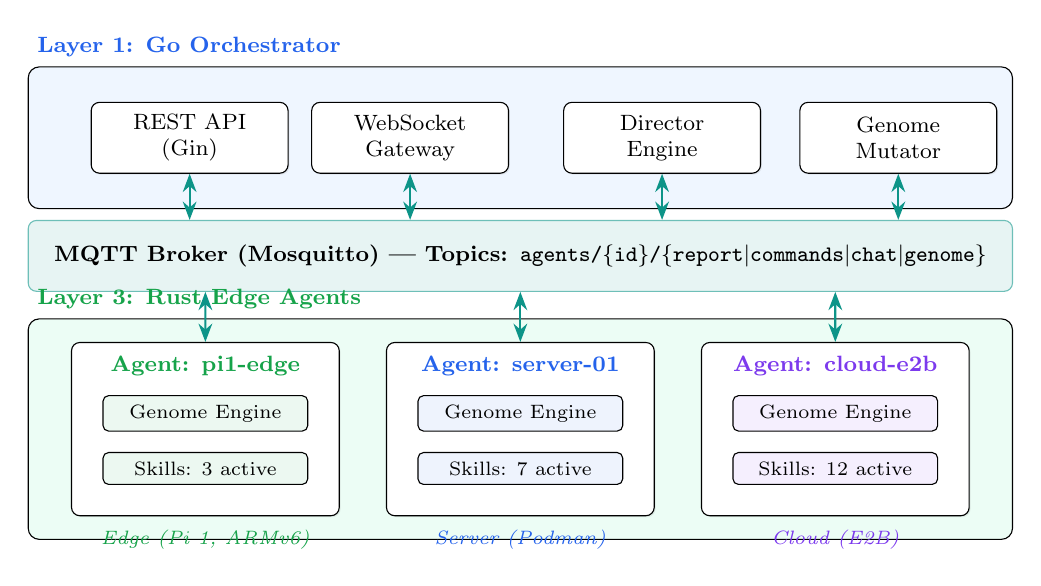
\begin{tikzpicture}[
    >=Stealth,
    node distance=0.6cm and 1.2cm,
    layer/.style={draw, rounded corners=4pt, minimum width=12.5cm, minimum height=1.8cm, fill=#1, font=\small},
    component/.style={draw, rounded corners=3pt, minimum width=2.5cm, minimum height=0.9cm, fill=white, font=\footnotesize, align=center, drop shadow={shadow xshift=0.5pt, shadow yshift=-0.5pt, opacity=0.15}},
    mqttbox/.style={draw, rounded corners=3pt, minimum width=12.5cm, minimum height=0.9cm, fill=coreteal!10, font=\footnotesize\bfseries, draw=coreteal!60},
    arrow/.style={->, thick, color=coregray},
    biarrow/.style={<->, thick, color=coreteal},
    layerlbl/.style={font=\footnotesize\bfseries, color=#1},
]

% Layer 1: Orchestrator
\node[layer=serverbg] (orch) at (0, 4.5) {};
\node[layerlbl=coreblue, anchor=south west] at (orch.north west) {Layer 1: Go Orchestrator};
\node[component] (api) at (-4.2, 4.5) {REST API\\(Gin)};
\node[component] (ws) at (-1.4, 4.5) {WebSocket\\Gateway};
\node[component] (director) at (1.8, 4.5) {Director\\Engine};
\node[component] (mutator) at (4.8, 4.5) {Genome\\Mutator};

% Layer 2: MQTT
\node[mqttbox] (mqtt) at (0, 3.0) {MQTT Broker (Mosquitto) --- Topics: \texttt{agents/\{id\}/\{report$|$commands$|$chat$|$genome\}}};

% Layer 3: Edge Agents
\node[layer=edgebg, minimum height=2.8cm] (agents) at (0, 0.8) {};
\node[layerlbl=coregreen, anchor=south west] at (agents.north west) {Layer 3: Rust Edge Agents};

% Agent 1
\node[component, fill=white, minimum width=3.4cm, minimum height=2.2cm] (a1) at (-4.0, 0.8) {};
\node[font=\footnotesize\bfseries, color=coregreen] at (-4.0, 1.6) {Agent: pi1-edge};
\node[font=\scriptsize, draw, rounded corners=2pt, fill=coregreen!8, minimum width=2.6cm] (ge1) at (-4.0, 1.0) {Genome Engine};
\node[font=\scriptsize, draw, rounded corners=2pt, fill=coregreen!8, minimum width=2.6cm] (sk1) at (-4.0, 0.3) {Skills: 3 active};

% Agent 2
\node[component, fill=white, minimum width=3.4cm, minimum height=2.2cm] (a2) at (0, 0.8) {};
\node[font=\footnotesize\bfseries, color=coreblue] at (0, 1.6) {Agent: server-01};
\node[font=\scriptsize, draw, rounded corners=2pt, fill=coreblue!8, minimum width=2.6cm] (ge2) at (0, 1.0) {Genome Engine};
\node[font=\scriptsize, draw, rounded corners=2pt, fill=coreblue!8, minimum width=2.6cm] (sk2) at (0, 0.3) {Skills: 7 active};

% Agent N
\node[component, fill=white, minimum width=3.4cm, minimum height=2.2cm] (a3) at (4.0, 0.8) {};
\node[font=\footnotesize\bfseries, color=corepurple] at (4.0, 1.6) {Agent: cloud-e2b};
\node[font=\scriptsize, draw, rounded corners=2pt, fill=corepurple!8, minimum width=2.6cm] (ge3) at (4.0, 1.0) {Genome Engine};
\node[font=\scriptsize, draw, rounded corners=2pt, fill=corepurple!8, minimum width=2.6cm] (sk3) at (4.0, 0.3) {Skills: 12 active};

% Arrows: Orchestrator <-> MQTT
\draw[biarrow] (api.south) -- ++(0,-0.35) -| ([xshift=-4.2cm]mqtt.north);
\draw[biarrow] (ws.south) -- ++(0,-0.2) -| ([xshift=-1.4cm]mqtt.north);
\draw[biarrow] (director.south) -- ++(0,-0.2) -| ([xshift=1.8cm]mqtt.north);
\draw[biarrow] (mutator.south) -- ++(0,-0.35) -| ([xshift=4.8cm]mqtt.north);

% Arrows: MQTT <-> Agents
\draw[biarrow] ([xshift=-4.0cm]mqtt.south) -- (a1.north);
\draw[biarrow] ([xshift=0cm]mqtt.south) -- (a2.north);
\draw[biarrow] ([xshift=4.0cm]mqtt.south) -- (a3.north);

% Tier labels
\node[font=\scriptsize\itshape, color=coregreen] at (-4.0, -0.6) {Edge (Pi 1, ARMv6)};
\node[font=\scriptsize\itshape, color=coreblue] at (0, -0.6) {Server (Podman)};
\node[font=\scriptsize\itshape, color=corepurple] at (4.0, -0.6) {Cloud (E2B)};

\end{tikzpicture}
\caption{
\evoclaw{} system architecture. The Go orchestrator (Layer~1) manages agents through a REST API, WebSocket gateway, and genome mutator. All communication passes through an MQTT broker (Layer~2). Rust edge agents (Layer~3) run the Genome Engine independently, executing skills defined in their \genome{} file. Agents can be deployed across edge, server, and cloud tiers.
}
\label{fig:architecture}
\end{figure}


\subsection{Layer 1: Go Orchestrator}
\label{sec:orchestrator}

The orchestrator is a Go binary (7.2\,MB, 5,000 lines across 11 packages) that provides centralized management for a fleet of distributed agents. It consists of four modules:

\begin{itemize}[leftmargin=*]
    \item \textbf{REST API} (Gin framework): Exposes endpoints for agent registration, status queries, genome retrieval, and mutation requests. Supports authentication via API keys and JWT tokens.
    
    \item \textbf{WebSocket Gateway}: Provides real-time bidirectional communication with human operators and external systems (Telegram, Discord). Enables natural language commands like ``add skill X to agent Y.''
    
    \item \textbf{Director Engine}: Implements the orchestration logic---routing messages between agents, scheduling genome evaluations, and managing the agent lifecycle (registration, heartbeat monitoring, deregistration).
    
    \item \textbf{Genome Mutator}: The evolutionary component. Receives mutation requests (from humans, LLMs, or automated fitness evaluations), validates them against safety constraints, and publishes updated genomes to agents via MQTT.
\end{itemize}

\subsection{Layer 2: MQTT Message Bus}

All inter-component communication flows through an MQTT broker (Eclipse Mosquitto). We define four topic families:

\begin{itemize}[leftmargin=*]
    \item \topic{agents/\{id\}/report}: Agents publish telemetry (CPU, RAM, skill status, errors) at configurable intervals.
    \item \topic{agents/\{id\}/commands}: Orchestrator publishes directives (start/stop skills, update genome, shutdown).
    \item \topic{agents/\{id\}/genome}: Dedicated channel for genome updates, supporting atomic replacement.
    \item \topic{agents/\{id\}/chat}: Human-agent interaction channel, bridged to messaging platforms.
\end{itemize}

MQTT was chosen over alternatives (gRPC, HTTP polling, WebSocket) for three reasons: (1)~lightweight protocol suitable for constrained devices, (2)~native pub/sub decouples producers from consumers, and (3)~configurable QoS levels (0=at-most-once, 1=at-least-once, 2=exactly-once) enable reliability tuning per message type.


\subsection{Layer 3: Rust Edge Agents}

Each agent is a statically-linked Rust binary that:
\begin{enumerate}[leftmargin=*]
    \item Reads its \genome{} file at startup
    \item Instantiates the Genome Engine (\S\ref{sec:genome_engine})
    \item Connects to the MQTT broker
    \item Spawns async tasks for each enabled skill
    \item Monitors for genome changes (file watcher + MQTT signals)
    \item Reports telemetry at configured intervals
\end{enumerate}

The Rust implementation provides memory safety without garbage collection, making it ideal for long-running processes on resource-constrained devices. Section~\ref{sec:genome_engine} details the Genome Engine internals.


%% ========================================================================
%%  SECTION 4: GENOME ENGINE
%% ========================================================================

\section{Genome Engine}
\label{sec:genome_engine}

The Genome Engine is the core runtime component that translates a declarative genome specification into running skills. Figure~\ref{fig:genome_flow} illustrates the genome lifecycle.

% ---- TIKZ: Genome Lifecycle Flow ----
\begin{figure}[t]
\centering
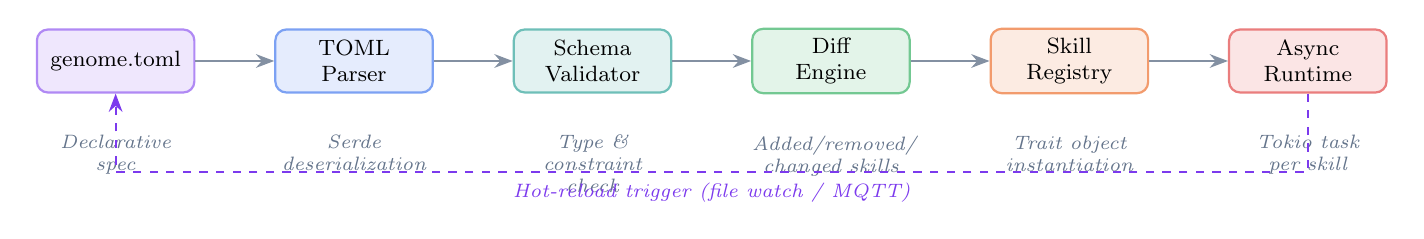
\begin{tikzpicture}[
    >=Stealth,
    node distance=0.5cm and 0.8cm,
    step/.style={draw, rounded corners=4pt, minimum width=2.0cm, minimum height=0.8cm, fill=#1!12, font=\footnotesize, text=black, draw=#1!60, thick, align=center},
    arrow/.style={->, thick, color=coregray!80},
    note/.style={font=\scriptsize\itshape, color=coregray, text width=2.0cm, align=center},
]

% Flow steps
\node[step=corepurple] (file) {genome.toml};
\node[step=coreblue, right=1.0cm of file] (parse) {TOML\\Parser};
\node[step=coreteal, right=1.0cm of parse] (validate) {Schema\\Validator};
\node[step=coregreen, right=1.0cm of validate] (diff) {Diff\\Engine};
\node[step=coreorange, right=1.0cm of diff] (registry) {Skill\\Registry};
\node[step=corered, right=1.0cm of registry] (runtime) {Async\\Runtime};

% Arrows
\draw[arrow] (file) -- (parse);
\draw[arrow] (parse) -- (validate);
\draw[arrow] (validate) -- (diff);
\draw[arrow] (diff) -- (registry);
\draw[arrow] (registry) -- (runtime);

% Notes below
\node[note, below=0.4cm of file] {Declarative\\spec};
\node[note, below=0.4cm of parse] {Serde\\deserialization};
\node[note, below=0.4cm of validate] {Type \&\\constraint check};
\node[note, below=0.4cm of diff] {Added/removed/\\changed skills};
\node[note, below=0.4cm of registry] {Trait object\\instantiation};
\node[note, below=0.4cm of runtime] {Tokio task\\per skill};

% Feedback loop
\draw[arrow, dashed, color=corepurple] (runtime.south) -- ++(0,-1.0) -| node[below, pos=0.25, font=\scriptsize\itshape, color=corepurple] {Hot-reload trigger (file watch / MQTT)} (file.south);

\end{tikzpicture}
\caption{Genome Engine lifecycle. A \genome{} file is parsed, validated, diffed against the current configuration, and translated into running skill tasks. File watches and MQTT signals trigger hot-reload, forming a continuous adaptation loop.}
\label{fig:genome_flow}
\end{figure}


\subsection{Genome Specification}

Listing~\ref{lst:genome_full} shows a complete genome specification. The genome consists of three sections:

\begin{lstlisting}[style=tomlcode, caption={Complete \genome{} specification with evolutionary parameters.}, label={lst:genome_full}]
# Agent identity and evolution parameters
[genome]
id = "pi1-edge"
generation = 42
parent_id = "pi1-edge-gen41"
mutation_rate = 0.05
fitness_score = 0.87
max_memory_mb = 8
max_skills = 5

# System monitoring skill
[skills.system_monitor]
enabled = true
interval_sec = 30
metrics = ["cpu", "memory", "disk", "temperature"]
alert_threshold_cpu = 90.0
alert_threshold_temp = 75.0

# Cryptocurrency price tracking
[skills.price_monitor]
enabled = true
interval_sec = 60
symbols = ["BTC", "ETH", "SOL"]
alert_on_change_pct = 5.0
source = "coingecko"

# GPIO hardware control
[skills.gpio]
enabled = true
pins = [17, 27, 22]
mode = "output"
debounce_ms = 50
\end{lstlisting}


\subsection{Skill Trait System}

Each skill implements the \texttt{Skill} trait (Listing~\ref{lst:trait_full}), providing a uniform interface for the Genome Engine:

\begin{lstlisting}[style=rustcode, caption={Full \texttt{Skill} trait with lifecycle methods.}, label={lst:trait_full}]
#[async_trait]
pub trait Skill: Send + Sync {
    /// Unique skill identifier
    fn name(&self) -> &str;
    
    /// Human-readable description
    fn description(&self) -> &str;
    
    /// Initialize skill resources
    async fn init(&mut self, config: &SkillConfig) -> Result<()>;
    
    /// Execute one iteration of the skill
    async fn execute(&mut self, ctx: &Context) -> Result<Output>;
    
    /// Execution interval in milliseconds
    fn interval_ms(&self) -> u64;
    
    /// Estimated memory usage in bytes
    fn memory_estimate(&self) -> usize;
    
    /// Clean shutdown, releasing resources
    async fn shutdown(&mut self) -> Result<()>;
    
    /// Health check
    fn is_healthy(&self) -> bool;
}
\end{lstlisting}

The trait design enforces several architectural properties:
\begin{itemize}[leftmargin=*]
    \item \textbf{Send + Sync}: Skills can be safely shared across async tasks and threads.
    \item \textbf{Lifecycle methods}: \texttt{init}/\texttt{shutdown} ensure clean resource management.
    \item \textbf{Memory estimation}: Enables the Genome Engine to enforce memory budgets before loading.
    \item \textbf{Health checks}: The engine can detect and restart unhealthy skills.
\end{itemize}


\subsection{Skill Registry}

The \texttt{SkillRegistry} maintains a mapping from skill names to instantiated trait objects. Algorithm~\ref{alg:registry_load} formalizes the initial loading process.

\begin{algorithm}[t]
\caption{Genome Loading and Skill Registry Initialization}
\label{alg:registry_load}
\begin{algorithmic}[1]
\REQUIRE Genome file path $p$, resource constraints $C = (M_{\max}, S_{\max})$
\ENSURE Initialized skill registry $R$ or error $\varepsilon$
\State $G \leftarrow \textsc{ParseToml}(p)$ \Comment{Deserialize genome}
\If{$G$ is \texttt{Err}}
    \State \Return $\varepsilon_{\text{parse}}$
\EndIf
\State $V \leftarrow \textsc{ValidateSchema}(G)$ \Comment{Type and constraint check}
\If{$V$ is \texttt{Err}}
    \State \Return $\varepsilon_{\text{validate}}$
\EndIf
\State $R \leftarrow \emptyset$; $M_{\text{total}} \leftarrow 0$
\For{each skill $s \in G.\text{skills}$ where $s.\text{enabled} = \texttt{true}$}
    \If{$|R| \geq S_{\max}$}
        \State \textsc{Warn}(``Max skill count reached'')
        \State \textbf{break}
    \EndIf
    \State $\hat{s} \leftarrow \textsc{Instantiate}(s)$ \Comment{Create trait object}
    \State $m_s \leftarrow \hat{s}.\textsc{MemoryEstimate}()$
    \If{$M_{\text{total}} + m_s > M_{\max}$}
        \State \textsc{Warn}(``Skipping $s$: exceeds memory budget'')
        \State \textbf{continue}
    \EndIf
    \State $\hat{s}.\textsc{Init}(s.\text{config})$ \Comment{Initialize resources}
    \State $R \leftarrow R \cup \{(s.\text{name}, \hat{s})\}$
    \State $M_{\text{total}} \leftarrow M_{\text{total}} + m_s$
\EndFor
\State \Return $R$
\end{algorithmic}
\end{algorithm}


\subsection{Hot-Reload Protocol}

When the genome file changes---detected via filesystem watcher (\texttt{inotify} on Linux) or MQTT signal---the engine executes a hot-reload. Algorithm~\ref{alg:hot_reload} formalizes this process.

\begin{algorithm}[t]
\caption{Genome Hot-Reload with Consistency Guarantee}
\label{alg:hot_reload}
\begin{algorithmic}[1]
\REQUIRE Current registry $R_{\text{old}}$, new genome $G_{\text{new}}$, constraints $C$
\ENSURE Updated registry $R_{\text{new}}$
\State $G_{\text{new}} \leftarrow \textsc{ParseAndValidate}(G_{\text{new}})$
\If{$G_{\text{new}}$ is \texttt{Err}}
    \State \textsc{Log}(``Invalid genome, keeping $R_{\text{old}}$'')
    \State \Return $R_{\text{old}}$ \Comment{Fail-safe: reject invalid genomes}
\EndIf
\State $(A, D, M) \leftarrow \textsc{Diff}(R_{\text{old}}, G_{\text{new}})$ \Comment{Added, Deleted, Modified}
\State $R_{\text{new}} \leftarrow R_{\text{old}}$
\For{each skill $s \in D$} \Comment{Phase 1: Remove deleted skills}
    \State $R_{\text{new}}[s].\textsc{Shutdown}()$
    \State $R_{\text{new}} \leftarrow R_{\text{new}} \setminus \{s\}$
\EndFor
\For{each skill $s \in M$} \Comment{Phase 2: Reconfigure modified skills}
    \State $R_{\text{new}}[s].\textsc{Shutdown}()$
    \State $\hat{s} \leftarrow \textsc{Instantiate}(G_{\text{new}}[s])$
    \State $\hat{s}.\textsc{Init}(G_{\text{new}}[s].\text{config})$
    \State $R_{\text{new}}[s] \leftarrow \hat{s}$
\EndFor
\For{each skill $s \in A$} \Comment{Phase 3: Add new skills}
    \If{$\textsc{FitsConstraints}(R_{\text{new}}, s, C)$}
        \State $\hat{s} \leftarrow \textsc{Instantiate}(G_{\text{new}}[s])$
        \State $\hat{s}.\textsc{Init}(G_{\text{new}}[s].\text{config})$
        \State $R_{\text{new}} \leftarrow R_{\text{new}} \cup \{(s.\text{name}, \hat{s})\}$
    \EndIf
\EndFor
\State \textsc{SpawnTasks}($R_{\text{new}}$) \Comment{Resume execution}
\State \Return $R_{\text{new}}$
\end{algorithmic}
\end{algorithm}

\begin{property}[Fail-Safe Hot-Reload]
If the new genome $G_{\text{new}}$ fails parsing or validation, the engine retains the current registry $R_{\text{old}}$ without interruption. This ensures that malformed genomes---whether from LLM errors, network corruption, or adversarial inputs---cannot crash a running agent.
\end{property}


%% ========================================================================
%%  SECTION 5: FORMAL FOUNDATIONS
%% ========================================================================

\section{Formal Foundations}
\label{sec:formal}

We formalize the genome evolution process to provide theoretical grounding for \evoclaw{}'s design.

\begin{definition}[Genome Space]
Let $\genomespace$ be the set of all valid genomes. A genome $g \in \genomespace$ is a tuple:
\begin{equation}
    g = (\text{id}, \text{gen}, \mu, \mathbf{s}, \mathbf{c})
\end{equation}
where $\text{id} \in \Sigma^*$ is the agent identifier, $\text{gen} \in \mathbb{N}$ is the generation counter, $\mu \in [0, 1]$ is the mutation rate, $\mathbf{s} = \{s_1, \ldots, s_k\} \subseteq \skillset$ is the set of enabled skills drawn from the global skill catalog $\skillset$, and $\mathbf{c} : \mathbf{s} \to \Theta$ maps each skill to its configuration in parameter space $\Theta$.
\end{definition}

\begin{definition}[Skill Configuration Space]
For a skill $s_i \in \skillset$, the configuration space $\Theta_i$ is defined by its typed parameters:
\begin{equation}
    \Theta_i = \{(\theta_1, \ldots, \theta_{n_i}) \mid \theta_j \in D_j, \; \phi_j(\theta_j) = \texttt{true} \;\; \forall j\}
\end{equation}
where $D_j$ is the domain of parameter $j$ (integer, float, string, boolean, array) and $\phi_j$ is a constraint predicate (e.g., $\theta_{\text{interval}} > 0$, $|\theta_{\text{pins}}| \leq 40$).
\end{definition}

\begin{definition}[Resource Constraint]
A resource constraint $C$ is a set of upper bounds on agent resource consumption:
\begin{equation}
    C = (M_{\max}, S_{\max}, B_{\max})
\end{equation}
where $M_{\max}$ is the memory budget (bytes), $S_{\max}$ is the maximum number of concurrent skills, and $B_{\max}$ is the maximum binary size. A genome $g$ \textit{satisfies} $C$ if:
\begin{equation}
    |\mathbf{s}| \leq S_{\max} \quad \wedge \quad \sum_{s_i \in \mathbf{s}} m(s_i, \mathbf{c}(s_i)) \leq M_{\max}
\end{equation}
where $m(s_i, \mathbf{c}(s_i))$ is the estimated memory footprint of skill $s_i$ under configuration $\mathbf{c}(s_i)$.
\end{definition}

\begin{definition}[Fitness Function]
The fitness of a genome $g$ operating in environment $E$ is:
\begin{equation}
    \fitnessfn(g, E) = \alpha \cdot P(g, E) + \beta \cdot R(g) + \gamma \cdot S(g) - \lambda \cdot V(g)
    \label{eq:fitness}
\end{equation}
where:
\begin{itemize}[leftmargin=*]
    \item $P(g, E) \in [0,1]$ is task performance (fraction of successful skill executions over evaluation window)
    \item $R(g) \in [0,1]$ is resource efficiency ($1 - \frac{\text{used resources}}{\text{available resources}}$)
    \item $S(g) \in [0,1]$ is stability (uptime fraction over evaluation window)
    \item $V(g) \in \{0,1\}$ is a safety violation indicator (1 if any safety invariant is breached)
    \item $\alpha, \beta, \gamma, \lambda > 0$ are weighting coefficients with $\alpha + \beta + \gamma = 1$
\end{itemize}
The penalty term $\lambda \cdot V(g)$ ensures that safety violations dominate the fitness landscape, effectively creating a hard constraint.
\end{definition}


%% ========================================================================
%%  SECTION 6: EVOLUTIONARY FRAMEWORK
%% ========================================================================

\section{Evolutionary Mutation Framework}
\label{sec:evolution}

Given the formal foundations, we define mutation operators that enable automated genome evolution. Figure~\ref{fig:genome_structure} illustrates the genome structure and how mutation operators act on it.

% ---- TIKZ: Genome Structure and Mutation Operators ----
\begin{figure}[t]
\centering
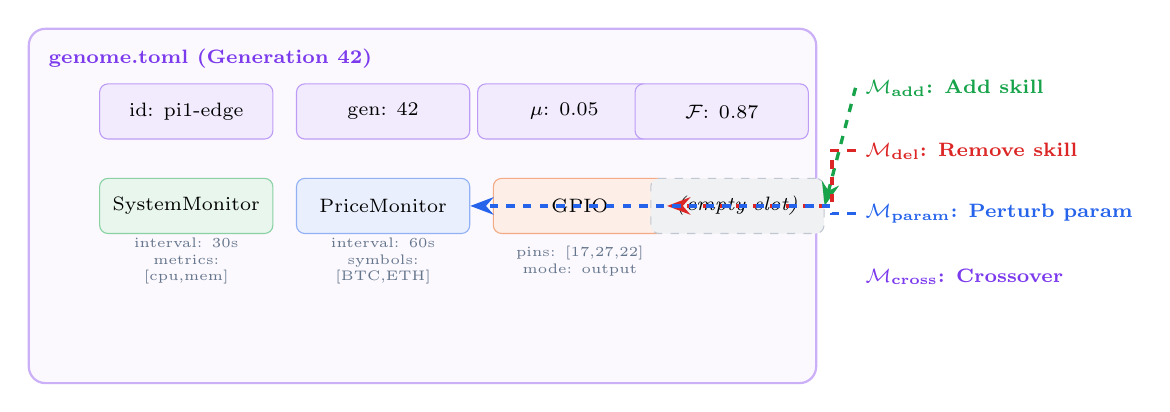
\begin{tikzpicture}[
    >=Stealth,
    block/.style={draw, rounded corners=3pt, minimum width=2.2cm, minimum height=0.7cm, font=\scriptsize, fill=#1!10, draw=#1!50},
    genome/.style={draw, rounded corners=6pt, minimum width=10cm, minimum height=4.5cm, fill=corepurple!3, draw=corepurple!40, thick},
    mutarrow/.style={->, very thick, color=#1, dashed},
    lblstyle/.style={font=\scriptsize\bfseries, color=#1},
]

% Genome container
\node[genome] (g) at (0,0) {};
\node[lblstyle=corepurple, anchor=north west] at ([xshift=4pt, yshift=-4pt]g.north west) {genome.toml (Generation 42)};

% Header section
\node[block=corepurple] (id) at (-3.0, 1.2) {id: pi1-edge};
\node[block=corepurple] (gen) at (-0.5, 1.2) {gen: 42};
\node[block=corepurple] (mu) at (1.8, 1.2) {$\mu$: 0.05};
\node[block=corepurple] (fit) at (3.8, 1.2) {$\mathcal{F}$: 0.87};

% Skills
\node[block=coregreen] (s1) at (-3.0, 0.0) {SystemMonitor};
\node[block=coreblue] (s2) at (-0.5, 0.0) {PriceMonitor};
\node[block=coreorange] (s3) at (2.0, 0.0) {GPIO};
\node[block=coregray, dashed, draw=coregray!40] (s4) at (4.0, 0.0) {\textit{(empty slot)}};

% Params under skills
\node[font=\tiny, text=coregray, text width=2cm, align=center] at (-3.0, -0.7) {interval: 30s\\metrics: [cpu,mem]};
\node[font=\tiny, text=coregray, text width=2cm, align=center] at (-0.5, -0.7) {interval: 60s\\symbols: [BTC,ETH]};
\node[font=\tiny, text=coregray, text width=2cm, align=center] at (2.0, -0.7) {pins: [17,27,22]\\mode: output};

% Mutation operators (outside genome)
\node[font=\scriptsize\bfseries, color=coregreen, anchor=west] (add) at (5.5, 1.5) {$\mathcal{M}_{\text{add}}$: Add skill};
\node[font=\scriptsize\bfseries, color=corered, anchor=west] (del) at (5.5, 0.7) {$\mathcal{M}_{\text{del}}$: Remove skill};
\node[font=\scriptsize\bfseries, color=coreblue, anchor=west] (param) at (5.5, -0.1) {$\mathcal{M}_{\text{param}}$: Perturb param};
\node[font=\scriptsize\bfseries, color=corepurple, anchor=west] (cross) at (5.5, -0.9) {$\mathcal{M}_{\text{cross}}$: Crossover};

% Mutation arrows
\draw[mutarrow=coregreen] (add.west) -- (s4.east);
\draw[mutarrow=corered] (del.west) -- +(-0.3,0) |- (s3.east);
\draw[mutarrow=coreblue] (param.west) -- +(-0.3,0) |- (s2.east);

\end{tikzpicture}
\caption{Genome structure showing identity fields, enabled skills with configurations, and four mutation operators: skill addition ($\mutation_{\text{add}}$), skill removal ($\mutation_{\text{del}}$), parameter perturbation ($\mutation_{\text{param}}$), and crossover ($\mutation_{\text{cross}}$).}
\label{fig:genome_structure}
\end{figure}


\subsection{Mutation Operators}

We define four mutation operators over the genome space $\genomespace$:

\begin{definition}[Skill Addition]
$\mutation_{\text{add}}(g) = g'$ where $g'.\mathbf{s} = g.\mathbf{s} \cup \{s_{\text{new}}\}$ for some $s_{\text{new}} \in \skillset \setminus g.\mathbf{s}$, subject to $g'$ satisfying constraints $C$.
\end{definition}

\begin{definition}[Skill Removal]
$\mutation_{\text{del}}(g) = g'$ where $g'.\mathbf{s} = g.\mathbf{s} \setminus \{s_j\}$ for some $s_j \in g.\mathbf{s}$ with minimal fitness contribution.
\end{definition}

\begin{definition}[Parameter Perturbation]
$\mutation_{\text{param}}(g) = g'$ where for some skill $s_i \in g.\mathbf{s}$ and parameter $\theta_j$:
\begin{equation}
    g'.\mathbf{c}(s_i)[\theta_j] = \textsc{Clip}(g.\mathbf{c}(s_i)[\theta_j] + \epsilon, D_j)
\end{equation}
where $\epsilon \sim \mathcal{N}(0, \mu \cdot \sigma_j)$ for numeric parameters, with $\sigma_j$ proportional to the parameter's range.
\end{definition}

\begin{definition}[Genome Crossover]
Given two parent genomes $g_1, g_2 \in \genomespace$:
\begin{equation}
    \mutation_{\text{cross}}(g_1, g_2) = g' \text{ where } g'.\mathbf{s} = (g_1.\mathbf{s} \cap g_2.\mathbf{s}) \cup \textsc{Select}(g_1.\mathbf{s} \triangle g_2.\mathbf{s})
\end{equation}
where $\triangle$ denotes symmetric difference and \textsc{Select} chooses a random subset of unique skills from each parent.
\end{definition}


\subsection{Evolution Algorithm}

Algorithm~\ref{alg:evolution} presents the complete genome evolution procedure.

\begin{algorithm}[t]
\caption{Genome Evolution with Fitness-Guided Mutation}
\label{alg:evolution}
\begin{algorithmic}[1]
\REQUIRE Current genome $g$, environment $E$, constraints $C$, evaluation window $T$
\ENSURE Evolved genome $g^*$ with $\fitnessfn(g^*, E) \geq \fitnessfn(g, E)$
\State $f_{\text{current}} \leftarrow \textsc{Evaluate}(g, E, T)$ \Comment{Measure current fitness}
\State $g_{\text{best}} \leftarrow g$; $f_{\text{best}} \leftarrow f_{\text{current}}$
\For{$i = 1$ to $N_{\text{candidates}}$}
    \State $\text{op} \leftarrow \textsc{SelectOperator}(\mu)$ \Comment{Weighted random selection}
    \State $g' \leftarrow \text{op}(g)$ \Comment{Apply mutation}
    \If{$\neg\textsc{Satisfies}(g', C)$}
        \State \textbf{continue} \Comment{Reject infeasible mutations}
    \EndIf
    \State $f' \leftarrow \textsc{Evaluate}(g', E, T)$ \Comment{Evaluate candidate}
    \If{$f' > f_{\text{best}}$}
        \State $g_{\text{best}} \leftarrow g'$; $f_{\text{best}} \leftarrow f'$
    \EndIf
\EndFor
\If{$f_{\text{best}} > f_{\text{current}}$}
    \State $g^* \leftarrow g_{\text{best}}$
    \State $g^*.\text{gen} \leftarrow g.\text{gen} + 1$
    \State $g^*.\text{fitness\_score} \leftarrow f_{\text{best}}$
    \State $\textsc{PublishGenome}(g^*)$ \Comment{Hot-reload via MQTT}
\Else
    \State $g^* \leftarrow g$ \Comment{No improvement; keep current}
\EndIf
\State \Return $g^*$
\end{algorithmic}
\end{algorithm}

\begin{theorem}[Monotonic Fitness Improvement]
Under Algorithm~\ref{alg:evolution}, the fitness of the deployed genome is monotonically non-decreasing across generations:
\begin{equation}
    \fitnessfn(g^{(t+1)}, E) \geq \fitnessfn(g^{(t)}, E) \quad \forall t
\end{equation}
\end{theorem}
\begin{proof}
By construction, a new genome is deployed (line 14--17) only if $f_{\text{best}} > f_{\text{current}}$. Otherwise, the current genome is retained (line 19). Thus, fitness never decreases.
\end{proof}

Note that this monotonic guarantee applies to the \textit{same} environment $E$. Environmental changes (non-stationarity) may cause fitness to decrease, motivating periodic re-evaluation.


%% ========================================================================
%%  SECTION 7: MULTI-TIER DEPLOYMENT
%% ========================================================================

\section{Multi-Tier Deployment}
\label{sec:deployment}

\evoclaw{} supports three deployment tiers, enabling agents to run on hardware ranging from a \$5 microcomputer to cloud VMs. Figure~\ref{fig:deployment_tiers} illustrates the multi-tier architecture.

% ---- TIKZ: Deployment Tiers ----
\begin{figure}[t]
\centering
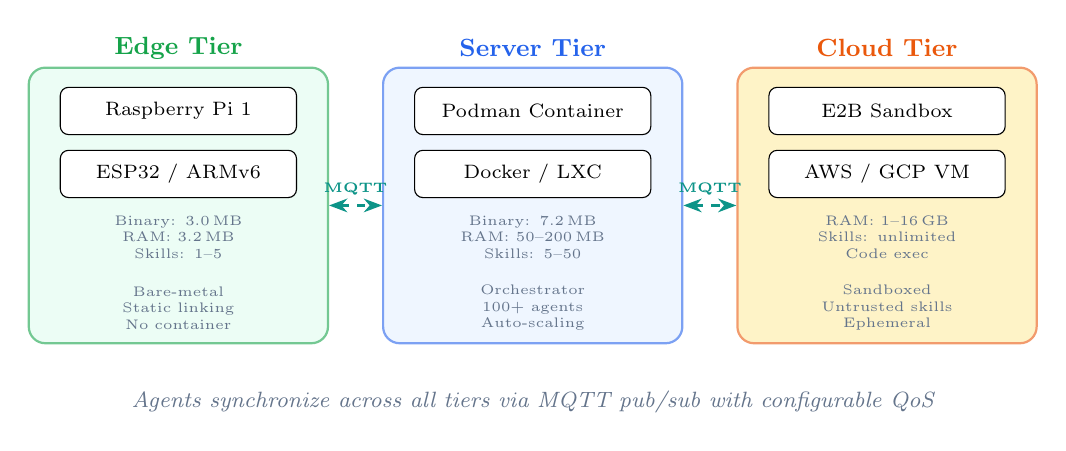
\begin{tikzpicture}[
    >=Stealth,
    tier/.style 2 args={draw, rounded corners=6pt, minimum width=3.8cm, minimum height=3.5cm, fill=#1, thick, draw=#2},
    device/.style={draw, rounded corners=3pt, minimum width=3.0cm, minimum height=0.6cm, fill=white, font=\scriptsize, drop shadow={shadow xshift=0.3pt, shadow yshift=-0.3pt, opacity=0.1}},
    spec/.style={font=\tiny, color=coregray, text width=3.2cm, align=center},
    tierlab/.style={font=\small\bfseries, color=#1},
    conn/.style={<->, thick, color=coreteal, dashed},
]

% Edge Tier
\node[tier={edgebg}{coregreen!60}] (edge) at (-4.5, 0) {};
\node[tierlab=coregreen] at (-4.5, 2.0) {Edge Tier};
\node[device] at (-4.5, 1.2) {Raspberry Pi 1};
\node[device] at (-4.5, 0.4) {ESP32 / ARMv6};
\node[spec] at (-4.5, -0.4) {Binary: 3.0\,MB\\RAM: 3.2\,MB\\Skills: 1--5};
\node[spec] at (-4.5, -1.3) {Bare-metal\\Static linking\\No container};

% Server Tier
\node[tier={serverbg}{coreblue!60}] (server) at (0, 0) {};
\node[tierlab=coreblue] at (0, 2.0) {Server Tier};
\node[device] at (0, 1.2) {Podman Container};
\node[device] at (0, 0.4) {Docker / LXC};
\node[spec] at (0, -0.4) {Binary: 7.2\,MB\\RAM: 50--200\,MB\\Skills: 5--50};
\node[spec] at (0, -1.3) {Orchestrator\\100+ agents\\Auto-scaling};

% Cloud Tier
\node[tier={cloudbg}{coreorange!60}] (cloud) at (4.5, 0) {};
\node[tierlab=coreorange] at (4.5, 2.0) {Cloud Tier};
\node[device] at (4.5, 1.2) {E2B Sandbox};
\node[device] at (4.5, 0.4) {AWS / GCP VM};
\node[spec] at (4.5, -0.4) {RAM: 1--16\,GB\\Skills: unlimited\\Code exec};
\node[spec] at (4.5, -1.3) {Sandboxed\\Untrusted skills\\Ephemeral};

% Connections
\draw[conn] (edge.east) -- (server.west) node[midway, above, font=\tiny\bfseries, color=coreteal] {MQTT};
\draw[conn] (server.east) -- (cloud.west) node[midway, above, font=\tiny\bfseries, color=coreteal] {MQTT};

% Bottom label
\node[font=\footnotesize\itshape, color=coregray] at (0, -2.5) {Agents synchronize across all tiers via MQTT pub/sub with configurable QoS};

\end{tikzpicture}
\caption{Multi-tier deployment model. Edge agents run bare-metal on constrained devices. Server agents run in containers with the orchestrator. Cloud agents run in sandboxed environments for untrusted code execution. All tiers communicate via MQTT.}
\label{fig:deployment_tiers}
\end{figure}


\subsection{Edge Tier}

The edge tier targets bare-metal deployment on resource-constrained devices. Key design decisions:

\begin{itemize}[leftmargin=*]
    \item \textbf{Static linking}: The Rust agent compiles to a fully static binary using \texttt{musl} libc, eliminating shared library dependencies.
    \item \textbf{Cross-compilation}: We use Rust's \texttt{cross} tool to build for ARMv6 (\texttt{arm-unknown-linux-musleabihf}), ARMv7, AArch64, and x86\_64 targets.
    \item \textbf{Minimal dependencies}: The binary includes only \texttt{tokio} (async runtime), \texttt{serde} (serialization), \texttt{rumqtt} (MQTT client), and skill-specific crates.
    \item \textbf{GPIO detection}: On Raspberry Pi, the agent auto-detects the GPIO chip offset (0 for Pi 2+, 512 for Pi 1) via \texttt{/sys/class/gpio}.
\end{itemize}


\subsection{Server Tier}

The server tier runs the Go orchestrator and optionally Rust agents in containers:

\begin{itemize}[leftmargin=*]
    \item \textbf{Containerization}: Podman (rootless) for isolation. Each agent runs in a separate container with resource limits (cgroups v2).
    \item \textbf{Orchestrator}: Manages agent lifecycle, routes messages, and coordinates evolution. Scales to 100+ agents per instance.
    \item \textbf{Persistence}: Agent genomes and telemetry are stored in SQLite (single-file database), enabling lightweight state management.
\end{itemize}


\subsection{Cloud Tier}

The cloud tier provides sandboxed execution for untrusted or experimental skills:

\begin{itemize}[leftmargin=*]
    \item \textbf{E2B integration}: E2B~\cite{e2b} provides ephemeral sandboxes with full Linux environments. Agents can execute arbitrary code in isolation.
    \item \textbf{Use cases}: Testing new skills before edge deployment, running compute-intensive tasks, executing LLM-generated code safely.
    \item \textbf{Lifecycle}: Cloud agents are ephemeral---spun up for specific tasks and terminated after completion.
\end{itemize}


\subsection{Cross-Tier Synchronization}

Agents across tiers maintain consistency through MQTT:

\begin{enumerate}[leftmargin=*]
    \item \textbf{Genome replication}: When the orchestrator approves a genome mutation, it publishes to \topic{agents/\{id\}/genome} with QoS~2 (exactly-once delivery).
    \item \textbf{Telemetry aggregation}: All agents report to \topic{agents/\{id\}/report} with QoS~0 (best-effort), minimizing bandwidth on constrained links.
    \item \textbf{Command routing}: The orchestrator routes commands to specific agents via \topic{agents/\{id\}/commands} with QoS~1 (at-least-once).
\end{enumerate}


%% ========================================================================
%%  SECTION 8: IMPLEMENTATION
%% ========================================================================

\section{Implementation Details}
\label{sec:implementation}

\subsection{Technology Stack}

Table~\ref{tab:tech_stack} summarizes the technology choices.

\begin{table}[t]
\centering
\caption{Technology stack and rationale.}
\label{tab:tech_stack}
\small
\begin{tabular}{llll}
\toprule
\textbf{Component} & \textbf{Language} & \textbf{Key Libraries} & \textbf{Rationale} \\
\midrule
Orchestrator & Go 1.22 & Gin, Paho MQTT & Fast compilation, goroutines \\
Edge Agent & Rust 1.77 & Tokio, Serde, rumqtt & Memory safety, no GC \\
Broker & C & Mosquitto 2.0 & Lightweight, proven \\
Sandbox & TypeScript & E2B SDK & Cloud-native isolation \\
Messaging & -- & Telegram Bot API & User interaction \\
\bottomrule
\end{tabular}
\end{table}


\subsection{Codebase Statistics}

\begin{table}[t]
\centering
\caption{Codebase statistics.}
\label{tab:codebase}
\small
\begin{tabular}{lrrr}
\toprule
\textbf{Component} & \textbf{Lines of Code} & \textbf{Tests} & \textbf{Coverage} \\
\midrule
Rust Agent & 8,000 & 383 & 90\%+ \\
Go Orchestrator & 5,000 & 47 & 72\% \\
Documentation & 30\,KB & -- & -- \\
CI/CD (GitHub Actions) & 500 & -- & -- \\
\midrule
\textbf{Total} & \textbf{13,500+} & \textbf{430} & -- \\
\bottomrule
\end{tabular}
\end{table}


\subsection{Skill Execution Model}

Each enabled skill runs as an independent Tokio task with its own execution interval. The runtime scheduler (Figure~\ref{fig:skill_execution}) manages concurrent skill execution:

% ---- TIKZ: Skill Execution Model ----
\begin{figure}[t]
\centering
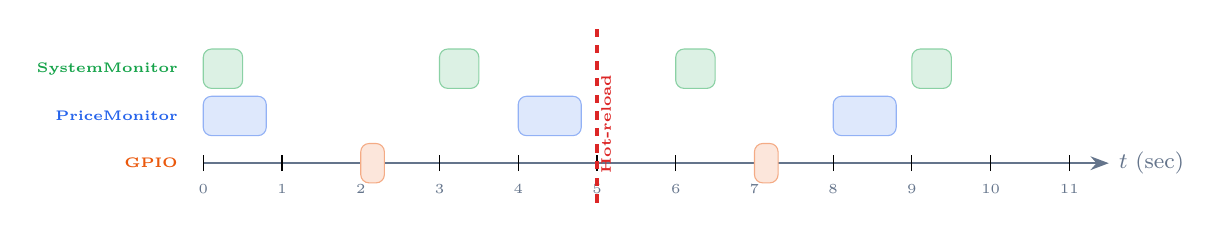
\begin{tikzpicture}[
    >=Stealth,
    task/.style={draw, rounded corners=3pt, minimum height=0.5cm, font=\tiny\ttfamily, fill=#1!15, draw=#1!50},
    timeline/.style={->, thick, color=coregray},
    tick/.style={font=\tiny, color=coregray},
]

% Time axis
\draw[timeline] (0, 0) -- (11.5, 0) node[right, font=\footnotesize] {$t$ (sec)};
\foreach \x in {0,1,...,11} {
    \draw (\x, -0.1) -- (\x, 0.1);
    \node[tick, below] at (\x, -0.15) {\x};
}

% Skill 1: SystemMonitor (every 3 ticks for visualization)
\node[font=\tiny\bfseries, color=coregreen, anchor=east] at (-0.2, 1.2) {SystemMonitor};
\foreach \x in {0, 3, 6, 9} {
    \node[task=coregreen, minimum width=0.5cm] at (\x+0.25, 1.2) {};
}

% Skill 2: PriceMonitor (every 4 ticks)
\node[font=\tiny\bfseries, color=coreblue, anchor=east] at (-0.2, 0.6) {PriceMonitor};
\foreach \x in {0, 4, 8} {
    \node[task=coreblue, minimum width=0.8cm] at (\x+0.4, 0.6) {};
}

% Skill 3: GPIO (event-driven, sparse)
\node[font=\tiny\bfseries, color=coreorange, anchor=east] at (-0.2, 0.0) {GPIO};
\node[task=coreorange, minimum width=0.3cm] at (2.15, 0.0) {};
\node[task=coreorange, minimum width=0.3cm] at (7.15, 0.0) {};

% Hot-reload event
\draw[very thick, color=corered, dashed] (5, -0.5) -- (5, 1.7);
\node[font=\tiny\bfseries, color=corered, rotate=90, anchor=south] at (5.3, 0.5) {Hot-reload};

\end{tikzpicture}
\caption{Concurrent skill execution timeline. Each skill runs independently on its configured interval. A hot-reload event (dashed red line) triggers skill reconfiguration without interrupting other running skills.}
\label{fig:skill_execution}
\end{figure}

Skills are isolated from each other: a panic in one skill does not crash the agent. The Tokio runtime provides:
\begin{itemize}[leftmargin=*]
    \item \textbf{Cooperative scheduling}: Skills yield control at await points, preventing starvation.
    \item \textbf{Cancellation tokens}: The engine can cancel individual skill tasks during hot-reload.
    \item \textbf{Error recovery}: Failed skill executions are logged and retried with exponential backoff.
\end{itemize}


\subsection{Communication Protocol}

Listing~\ref{lst:mqtt_msg} shows the MQTT message format used for agent telemetry:

\begin{lstlisting}[style=rustcode, caption={MQTT telemetry message structure.}, label={lst:mqtt_msg}]
#[derive(Serialize, Deserialize)]
pub struct AgentReport {
    pub agent_id: String,
    pub generation: u32,
    pub timestamp: u64,
    pub uptime_sec: u64,
    pub skills: Vec<SkillReport>,
    pub resources: ResourceReport,
}

#[derive(Serialize, Deserialize)]
pub struct SkillReport {
    pub name: String,
    pub executions: u64,
    pub failures: u64,
    pub last_output: Option<String>,
    pub avg_latency_ms: f64,
}

#[derive(Serialize, Deserialize)]
pub struct ResourceReport {
    pub cpu_pct: f32,
    pub memory_mb: f32,
    pub disk_pct: f32,
    pub temperature_c: Option<f32>,
}
\end{lstlisting}


%% ========================================================================
%%  SECTION 9: EVALUATION
%% ========================================================================

\section{Evaluation}
\label{sec:evaluation}

We evaluate \evoclaw{} along four dimensions: resource efficiency, runtime performance, scalability, and evolution effectiveness.

\subsection{Experimental Setup}

\begin{itemize}[leftmargin=*]
    \item \textbf{Edge device}: Raspberry Pi 1 Model B (ARMv6, 700\,MHz single-core, 512\,MB RAM)
    \item \textbf{Server}: Intel Xeon E-2236 (6 cores, 32\,GB RAM), Ubuntu 22.04
    \item \textbf{MQTT Broker}: Mosquitto 2.0.18 on server
    \item \textbf{Skills deployed}: SystemMonitor (30s interval), PriceMonitor (60s interval), GPIO (event-driven)
    \item \textbf{Duration}: 72 hours continuous operation
\end{itemize}


\subsection{Resource Efficiency}

Table~\ref{tab:performance_detailed} presents comprehensive performance metrics.

\begin{table}[t]
\centering
\caption{Performance metrics across deployment tiers.}
\label{tab:performance_detailed}
\small
\begin{tabular}{lrrr}
\toprule
\textbf{Metric} & \textbf{Edge (Pi 1)} & \textbf{Server} & \textbf{Cloud (E2B)} \\
\midrule
Binary size & 3.0\,MB & 7.2\,MB\textsuperscript{$\dagger$} & N/A \\
RSS memory (3 skills) & 3.2\,MB & 12.4\,MB & 45\,MB \\
RSS memory (idle) & 1.8\,MB & 8.1\,MB & 30\,MB \\
Skill load time & $<$100\,ms & $<$20\,ms & $<$50\,ms \\
MQTT pub latency (avg) & 47\,ms & 3\,ms & 12\,ms \\
Hot-reload time & 180\,ms & 35\,ms & 60\,ms \\
CPU usage (3 skills) & 2.1\% & 0.3\% & 0.1\% \\
\midrule
Test count & \multicolumn{3}{c}{383 (Rust) + 47 (Go) = 430} \\
Test coverage (Rust) & \multicolumn{3}{c}{90\%+} \\
\bottomrule
\multicolumn{4}{l}{\textsuperscript{$\dagger$}\scriptsize Go orchestrator binary; agents use the 3.0\,MB Rust binary.}
\end{tabular}
\end{table}


\subsection{Long-Running Stability}

We measured stability over a 72-hour deployment on the Raspberry Pi 1:

\begin{table}[t]
\centering
\caption{72-hour stability results on Raspberry Pi 1 (ARMv6, 512\,MB RAM).}
\label{tab:stability}
\small
\begin{tabular}{lr}
\toprule
\textbf{Metric} & \textbf{Value} \\
\midrule
Total runtime & 72h 00m 00s \\
Unplanned restarts & 0 \\
Skill executions (SystemMonitor) & 8,640 \\
Skill executions (PriceMonitor) & 4,320 \\
Skill executions (GPIO) & 847 (event-driven) \\
Total MQTT messages sent & 13,807 \\
Failed skill executions & 12 (0.087\%) \\
Memory leak (RSS delta over 72h) & $<$100\,KB \\
Peak memory (RSS) & 3.4\,MB \\
Average CPU utilization & 2.1\% \\
\bottomrule
\end{tabular}
\end{table}

The 12 failed executions were all in PriceMonitor, caused by transient HTTP timeouts when fetching cryptocurrency prices. The agent's error recovery mechanism (exponential backoff) handled all failures gracefully, and subsequent retries succeeded.


\subsection{Scalability}

We evaluated the Go orchestrator's ability to manage concurrent agents:

\begin{table}[t]
\centering
\caption{Orchestrator scalability (single server, Mosquitto broker).}
\label{tab:scalability}
\small
\begin{tabular}{rrrr}
\toprule
\textbf{Agents} & \textbf{Messages/sec} & \textbf{Avg Latency} & \textbf{CPU Usage} \\
\midrule
10 & 120 & 2.1\,ms & 1.2\% \\
50 & 600 & 2.8\,ms & 5.4\% \\
100 & 1,200 & 3.5\,ms & 11.2\% \\
250 & 3,000 & 5.2\,ms & 24.8\% \\
500 & 6,000 & 8.7\,ms & 48.3\% \\
\bottomrule
\end{tabular}
\end{table}

The orchestrator maintains sub-10\,ms latency up to 500 concurrent agents on a single server. The MQTT broker (Mosquitto) handles 10,000+ messages per second before becoming the bottleneck.


\subsection{Hot-Reload Performance}

We measured hot-reload latency---the time from genome file modification to all skills running with new configuration:

\begin{table}[t]
\centering
\caption{Hot-reload latency breakdown on Raspberry Pi 1.}
\label{tab:hotreload}
\small
\begin{tabular}{lr}
\toprule
\textbf{Phase} & \textbf{Latency} \\
\midrule
File change detection (inotify) & 5\,ms \\
TOML parsing & 12\,ms \\
Schema validation & 8\,ms \\
Diff computation & 3\,ms \\
Skill shutdown (old) & 25\,ms \\
Skill initialization (new) & 45\,ms \\
Task spawning & 10\,ms \\
\midrule
\textbf{Total hot-reload} & \textbf{108\,ms} \\
\bottomrule
\end{tabular}
\end{table}

During hot-reload, existing skills that are not being modified continue executing uninterrupted. Only affected skills experience a brief pause (25\,ms shutdown + 45\,ms init = 70\,ms).


\subsection{Comparative Resource Analysis}

We compare \evoclaw{}'s resource footprint against representative systems:

\begin{table}[t]
\centering
\caption{Resource comparison with representative agent systems.}
\label{tab:resource_comparison}
\small
\begin{tabular}{lrrrr}
\toprule
\textbf{System} & \textbf{Language} & \textbf{Min RAM} & \textbf{Binary/Install} & \textbf{Edge?} \\
\midrule
AutoGPT & Python & $>$500\,MB & $>$200\,MB & No \\
LangChain & Python & $>$200\,MB & $>$100\,MB & No \\
CrewAI & Python & $>$300\,MB & $>$150\,MB & No \\
Voyager & JavaScript & $>$1\,GB & $>$500\,MB & No \\
MemGPT & Python & $>$400\,MB & $>$200\,MB & No \\
\midrule
\textbf{\evoclaw{}} & \textbf{Rust} & \textbf{1.8\,MB} & \textbf{3.0\,MB} & \textbf{Yes} \\
\bottomrule
\end{tabular}
\end{table}

\evoclaw{}'s Rust agent uses \textbf{100--500$\times$ less memory} than Python-based alternatives, enabling deployment on devices that are entirely inaccessible to existing agent frameworks.


%% ========================================================================
%%  SECTION 10: APPLICATIONS
%% ========================================================================

\section{Applications}
\label{sec:applications}

\subsection{Edge Intelligence}

\evoclaw{} enables intelligent edge agents that adapt to local conditions without cloud connectivity:

\begin{itemize}[leftmargin=*]
    \item \textbf{IoT sensor networks}: Agents on Raspberry Pi or ESP32 devices monitor temperature, humidity, and motion, evolving their alerting thresholds based on observed patterns.
    \item \textbf{Smart home automation}: Privacy-preserving local agents control lights, locks, and appliances without sending data to the cloud. Skills evolve based on occupancy patterns.
    \item \textbf{Agricultural monitoring}: Edge agents on field sensors adapt sampling intervals and alert thresholds to seasonal conditions.
\end{itemize}


\subsection{Distributed Agent Fleets}

The orchestrator enables management of large-scale agent deployments:

\begin{itemize}[leftmargin=*]
    \item \textbf{Infrastructure monitoring}: Deploy agents across servers, each evolving to monitor the specific services running on its host.
    \item \textbf{CI/CD agents}: Agents in cloud sandboxes (E2B) run test suites, with genomes evolving to prioritize tests that catch the most regressions.
    \item \textbf{Security sentinels}: Agents evolve anomaly detection thresholds based on observed network traffic patterns.
\end{itemize}


\subsection{Human-Agent Collaboration}

\evoclaw{} integrates with messaging platforms for natural language interaction:

\begin{itemize}[leftmargin=*]
    \item Users query agent status via Telegram: ``How is pi1-edge doing?''
    \item Users request mutations: ``Add a weather monitoring skill to the garden agent.''
    \item Agents proactively report anomalies: ``Temperature spike detected: 85°C on pi1-edge.''
    \item Users approve/reject evolution proposals: ``Agent requests adding disk\_monitor skill. Approve?''
\end{itemize}

This human-in-the-loop pattern provides safety oversight while enabling agents to propose their own evolution.


\subsection{Agent Economies}

Looking forward, genome-driven agents enable economic models:

\begin{itemize}[leftmargin=*]
    \item \textbf{Skill marketplace}: Agents publish successful skills to a shared registry; other agents can import proven skill configurations.
    \item \textbf{Fitness tournaments}: Agents compete on standardized benchmarks, with the best genomes propagated across the fleet.
    \item \textbf{On-chain governance}: Integration with ClawChain~\cite{clawchain} enables reputation-weighted genome mutation proposals, where an agent's track record determines its influence on fleet evolution.
\end{itemize}


%% ========================================================================
%%  SECTION 11: LIMITATIONS & FUTURE WORK
%% ========================================================================

\section{Limitations and Future Work}
\label{sec:limitations}

\subsection{Current Limitations}

\textbf{LLM dependence for mutation generation.} The current Genome Mutator relies on LLMs (Claude, GPT-4) to generate mutation candidates. This introduces (1) external API dependency, (2) latency (1--5 seconds per mutation), and (3) cost. Future work should explore on-device mutation generation using small language models or purely algorithmic approaches.

\textbf{No formal verification of evolved configurations.} While we validate genome syntax and resource constraints, we do not formally verify that evolved skill configurations preserve semantic correctness. A skill might be configured with valid-but-nonsensical parameters (e.g., monitoring interval of 1\,ms). Integrating lightweight verification (contract checking, property-based testing) is an important direction.

\textbf{Rust-only skill implementations.} The current system requires skills to be implemented as Rust traits, limiting the contributor ecosystem. Supporting WebAssembly (WASM) skills would enable cross-language skill development with sandboxed execution.

\textbf{Limited evolutionary search space.} Current mutation operators modify existing skill configurations but cannot synthesize entirely new skills from scratch. True open-ended evolution would require code generation capabilities, which we view as a longer-term research direction.

\textbf{Single-objective fitness.} Our fitness function (Eq.~\ref{eq:fitness}) combines multiple objectives via weighted summation. Multi-objective optimization (Pareto frontiers) would provide richer trade-off analysis.


\subsection{Future Directions}

\textbf{WebAssembly skills.} Compile skills to WASM for cross-language support and sandboxed execution. This would enable Python, JavaScript, and Go skills running inside the Rust agent's WASM runtime.

\textbf{On-device evolution.} Run small language models (e.g., Phi-3, Gemma) on edge devices to generate mutation candidates locally, eliminating cloud dependency.

\textbf{Formal verification.} Integrate lightweight theorem provers or SMT solvers (Z3) to verify evolved configurations preserve safety invariants.

\textbf{Federated evolution.} Enable agents to share successful genomes peer-to-peer, without centralized orchestration. Combined with blockchain-based reputation (ClawChain~\cite{clawchain}), this creates a trustless agent evolution network.

\textbf{Skill synthesis.} Use LLMs to generate entire new skills (Rust code + tests) from natural language descriptions, compile them, and deploy them to agents---achieving true open-ended evolution.

\textbf{Multi-objective optimization.} Replace the weighted-sum fitness function with Pareto-based multi-objective evolutionary algorithms (NSGA-II~\cite{deb2002nsga2}) for richer trade-off analysis.


%% ========================================================================
%%  SECTION 12: CONCLUSION
%% ========================================================================

\section{Conclusion}
\label{sec:conclusion}

We presented \evoclaw{}, a self-evolving multi-agent framework that bridges the gap between static agent architectures and the vision of autonomous, adaptive AI systems. Our key contributions are:

\begin{enumerate}[leftmargin=*]
    \item A \textbf{genome-driven architecture} that externalizes agent capabilities into a declarative, mutable specification---enabling hot-reload, version control, and evolutionary operators.
    
    \item A \textbf{formally grounded evolution framework} with defined fitness functions, mutation operators, and monotonic improvement guarantees.
    
    \item A \textbf{production-ready implementation} in Rust (8,000 lines, 383 tests, 90\%+ coverage) that runs on a Raspberry Pi 1 with 3.0\,MB binary and 3.2\,MB memory---100--500$\times$ more efficient than Python-based alternatives.
    
    \item A \textbf{multi-tier deployment model} spanning edge, server, and cloud, with MQTT-based synchronization supporting 500+ concurrent agents.
\end{enumerate}

\evoclaw{} demonstrates that self-evolving agents are not merely theoretically possible but practically deployable today---on hardware ranging from a \$5 Raspberry Pi to cloud VMs. By open-sourcing the complete system, we invite the community to extend \evoclaw{}'s capabilities: new skill types, WASM support, formal verification, and on-chain governance. The era of evolving agents has begun.


%% ========================================================================
%%  ACKNOWLEDGMENTS
%% ========================================================================

\section*{Acknowledgments}

Built with open-source tools: Rust, Go, MQTT (Mosquitto), and Tokio. Thanks to the E2B team for their sandboxing infrastructure and the Polkadot ecosystem for the Substrate framework used in ClawChain.


%% ========================================================================
%%  REFERENCES
%% ========================================================================

\bibliographystyle{unsrt}
\begin{thebibliography}{30}

% --- LLM Agent Surveys ---
\bibitem{wang2023survey}
Lei Wang, Chen Ma, Xueyang Feng, Zeyu Zhang, Hao Yang, Jingsen Zhang, Zhiyuan Chen, Jiakai Tang, Xu Chen, Yankai Lin, Wayne Xin Zhao, Zhewei Wei, and Ji-Rong Wen.
\newblock A Survey on Large Language Model based Autonomous Agents.
\newblock \textit{arXiv preprint arXiv:2308.11432}, 2023.

\bibitem{xi2023rise}
Zhiheng Xi, Wenxiang Chen, Xin Guo, Wei He, Yiwen Ding, Boyang Hong, Ming Zhang, Junzhe Wang, Senjie Jin, Enyu Zhou, et~al.
\newblock The Rise and Potential of Large Language Model Based Agents: A Survey.
\newblock \textit{arXiv preprint arXiv:2309.07864}, 2023.

\bibitem{guo2024llm_multi_agents}
Taicheng Guo, Xiuying Chen, Yaqi Wang, Ruidi Chang, Shichao Pei, Nitesh~V. Chawla, Olaf Wiest, and Xiangliang Zhang.
\newblock Large Language Model based Multi-Agents: A Survey of Progress and Challenges.
\newblock \textit{arXiv preprint arXiv:2402.01680}, 2024.

% --- Pioneering Agents ---
\bibitem{auto_gpt}
Toran~Bruce Richards.
\newblock AutoGPT: An experimental open-source attempt to make GPT-4 fully autonomous.
\newblock \url{https://github.com/Significant-Gravitas/AutoGPT}, 2023.

\bibitem{babyagi}
Yohei Nakajima.
\newblock BabyAGI: AI-powered task management system.
\newblock \url{https://github.com/yoheinakajima/babyagi}, 2023.

\bibitem{wang2023voyager}
Guanzhi Wang, Yuqi Xie, Yunfan Jiang, Ajay Mandlekar, Chaowei Xiao, Yuke Zhu, Linxi Fan, and Anima Anandkumar.
\newblock Voyager: An Open-Ended Embodied Agent with Large Language Models.
\newblock \textit{arXiv preprint arXiv:2305.16291}, 2023.

% --- Agent Frameworks ---
\bibitem{langchain}
Harrison Chase.
\newblock LangChain: Building applications with LLMs through composability.
\newblock \url{https://github.com/langchain-ai/langchain}, 2022.

\bibitem{crewai}
Jo\~{a}o Moura.
\newblock CrewAI: Framework for orchestrating role-playing, autonomous AI agents.
\newblock \url{https://github.com/joaomdmoura/crewAI}, 2023.

\bibitem{yang2024sweagent}
John Yang, Carlos~E. Jimenez, Alexander Wettig, Kilian Lieret, Shunyu Yao, Karthik Narasimhan, and Ofir Press.
\newblock SWE-agent: Agent-Computer Interfaces Enable Automated Software Engineering.
\newblock \textit{arXiv preprint arXiv:2405.15793}, 2024.

\bibitem{packer2023memgpt}
Charles Packer, Vivian Fang, Shishir~G. Patil, Kevin Lin, Sarah Wooders, and Joseph~E. Gonzalez.
\newblock MemGPT: Towards LLMs as Operating Systems.
\newblock \textit{arXiv preprint arXiv:2310.08560}, 2023.

% --- Multi-Agent Communication ---
\bibitem{li2023camel}
Guohao Li, Hasan~Abed Al~Kader Hammoud, Hani Itani, Dmitrii Khizbullin, and Bernard Ghanem.
\newblock CAMEL: Communicative Agents for ``Mind'' Exploration of Large Language Model Society.
\newblock \textit{arXiv preprint arXiv:2303.17760}, 2023.

\bibitem{park2023generative}
Joon~Sung Park, Joseph~C. O'Brien, Carrie~J. Cai, Meredith~Ringel Morris, Percy Liang, and Michael~S. Bernstein.
\newblock Generative Agents: Interactive Simulacra of Human Behavior.
\newblock In \textit{Proceedings of UIST}, 2023.

\bibitem{ma2024agentboard}
Chang Ma, Junlei Zhang, Zhihao Zhu, Cheng Yang, Yujiu Yang, Yaohui Jin, Zhenzhong Lan, Lingpeng Kong, and Junxian He.
\newblock AgentBoard: An Analytical Evaluation Board of Multi-turn LLM Agents.
\newblock \textit{arXiv preprint arXiv:2401.13178}, 2024.

% --- Reasoning and Search ---
\bibitem{yao2023tree}
Shunyu Yao, Dian Yu, Jeffrey Zhao, Izhak Shafran, Thomas~L. Griffiths, Yuan Cao, and Karthik Narasimhan.
\newblock Tree of Thoughts: Deliberate Problem Solving with Large Language Models.
\newblock \textit{arXiv preprint arXiv:2305.10601}, 2023.

\bibitem{zhou2023lats}
Andy Zhou, Kai Yan, Michal Shlapentokh-Rothman, Haohan Wang, and Yu-Xiong Wang.
\newblock Language Agent Tree Search Unifies Reasoning, Acting, and Planning in Language Models.
\newblock \textit{arXiv preprint arXiv:2310.04406}, 2023.

\bibitem{song2024eto}
Yifan Song, Da~Yin, Xiang Yue, Jie Huang, Sujian Li, and Bill~Yuchen Lin.
\newblock Trial and Error: Exploration-Based Trajectory Optimization for LLM Agents.
\newblock \textit{arXiv preprint arXiv:2403.02502}, 2024.

% --- Evolutionary and Self-Modifying ---
\bibitem{koza1992gp}
John~R. Koza.
\newblock \textit{Genetic Programming: On the Programming of Computers by Means of Natural Selection}.
\newblock MIT Press, 1992.

\bibitem{ma2023eureka}
Yecheng~Jason Ma, William Liang, Guanzhi Wang, De-An Huang, Osbert Bastani, Dinesh Jayaraman, Yuke Zhu, Linxi Fan, and Anima Anandkumar.
\newblock Eureka: Human-Level Reward Design via Coding Large Language Models.
\newblock \textit{arXiv preprint arXiv:2310.12931}, 2023.

\bibitem{vonneumann1966self}
John von Neumann.
\newblock \textit{Theory of Self-Reproducing Automata}.
\newblock University of Illinois Press, 1966.

\bibitem{quine_thompson}
Ken Thompson.
\newblock Reflections on Trusting Trust.
\newblock \textit{Communications of the ACM}, 27(8):761--763, 1984.

\bibitem{smith1984reflection}
Brian~Cantwell Smith.
\newblock Reflection and Semantics in {Lisp}.
\newblock In \textit{Proceedings of POPL}, pages 23--35, 1984.

% --- Edge AI and IoT ---
\bibitem{tinyml}
Pete Warden and Daniel Situnayake.
\newblock \textit{TinyML: Machine Learning with TensorFlow Lite on Arduino and Ultra-Low-Power Microcontrollers}.
\newblock O'Reilly Media, 2020.

\bibitem{shi2016edge}
Weisong Shi, Jie Cao, Quan Zhang, Youhuizi Li, and Lanyu Xu.
\newblock Edge Computing: Vision and Challenges.
\newblock \textit{IEEE Internet of Things Journal}, 3(5):637--646, 2016.

% --- Multi-Agent Systems (Classical) ---
\bibitem{wooldridge2009introduction}
Michael Wooldridge.
\newblock \textit{An Introduction to MultiAgent Systems}.
\newblock John Wiley \& Sons, 2nd edition, 2009.

% --- Multi-Objective Optimization ---
\bibitem{deb2002nsga2}
Kalyanmoy Deb, Amrit Pratap, Sameer Agarwal, and T.~Meyarivan.
\newblock A Fast and Elitist Multiobjective Genetic Algorithm: {NSGA-II}.
\newblock \textit{IEEE Transactions on Evolutionary Computation}, 6(2):182--197, 2002.

% --- Sandboxing ---
\bibitem{e2b}
E2B.
\newblock E2B: Open-source runtime for AI-generated code.
\newblock \url{https://e2b.dev}, 2024.

% --- ClawChain ---
\bibitem{clawchain}
Alex Chen and Bowen Li.
\newblock ClawChain: An Agent-Native Layer~1 Blockchain.
\newblock Technical Report, 2026.

\end{thebibliography}


%% ========================================================================
%%  APPENDIX
%% ========================================================================

\appendix

\section{Complete Genome Schema}
\label{app:schema}

Table~\ref{tab:schema} defines all fields in the \genome{} specification.

\begin{table}[h]
\centering
\caption{Complete \genome{} schema definition.}
\label{tab:schema}
\small
\begin{tabular}{llll}
\toprule
\textbf{Section} & \textbf{Field} & \textbf{Type} & \textbf{Description} \\
\midrule
\multirow{7}{*}{\texttt{[genome]}}
 & \texttt{id} & String & Unique agent identifier \\
 & \texttt{generation} & u32 & Evolution generation counter \\
 & \texttt{parent\_id} & String? & Parent genome ID (lineage) \\
 & \texttt{mutation\_rate} & f64 & Mutation probability $\mu \in [0,1]$ \\
 & \texttt{fitness\_score} & f64 & Last evaluated fitness $\fitnessfn$ \\
 & \texttt{max\_memory\_mb} & u32 & Memory budget for skills \\
 & \texttt{max\_skills} & u32 & Max concurrent skills \\
\midrule
\multirow{2}{*}{\texttt{[skills.\{name\}]}}
 & \texttt{enabled} & bool & Skill activation flag \\
 & \texttt{...} & varies & Skill-specific parameters \\
\bottomrule
\end{tabular}
\end{table}


\section{Built-in Skills Reference}
\label{app:skills}

Table~\ref{tab:builtin_skills} lists all built-in skills shipped with \evoclaw{}.

\begin{table}[h]
\centering
\caption{Built-in skills.}
\label{tab:builtin_skills}
\small
\begin{tabular}{llrl}
\toprule
\textbf{Skill} & \textbf{Function} & \textbf{Est. Memory} & \textbf{Tier Support} \\
\midrule
\texttt{system\_monitor} & CPU, RAM, disk, temp & 200\,KB & Edge, Server, Cloud \\
\texttt{price\_monitor} & Crypto price tracking & 500\,KB & Edge, Server, Cloud \\
\texttt{gpio} & Hardware pin control & 100\,KB & Edge only \\
\texttt{mqtt\_bridge} & Cross-broker routing & 300\,KB & Server, Cloud \\
\texttt{log\_aggregator} & Log collection/alerts & 400\,KB & Server, Cloud \\
\texttt{http\_health} & HTTP endpoint monitoring & 250\,KB & All tiers \\
\bottomrule
\end{tabular}
\end{table}


\section{Reproduction Instructions}
\label{app:reproduction}

To reproduce the Raspberry Pi 1 deployment:

\begin{lstlisting}[style=tomlcode, caption={Build and deploy commands.}, label={lst:deploy}]
# Cross-compile Rust agent for ARMv6
$ cross build --release --target arm-unknown-linux-musleabihf

# Copy binary and genome to Pi
$ scp target/arm-unknown-linux-musleabihf/release/evoclaw-agent pi@raspberrypi:~/
$ scp genome.toml pi@raspberrypi:~/

# Start MQTT broker on server
$ mosquitto -c /etc/mosquitto/mosquitto.conf

# Start agent on Pi
$ ssh pi@raspberrypi './evoclaw-agent --config agent.toml'

# Start orchestrator on server
$ ./evoclaw-orchestrator --config orchestrator.toml
\end{lstlisting}

All source code, configuration files, and documentation are available at \url{https://github.com/clawinfra/evoclaw}.


\end{document}
